
\section{Analisa dan Perancangan}
\subsection{\textit{Bussiness Engineering}}
Ketika bisnis digabungkan dengan teknologi atau yang sering disebut \textit{e-commerce}, hal yang sekedar pertukaran barang bertransformasi menjadi sebuah sistem interaktif yang kompleks dimana tujuan utamanya adalah menarik pengunjung/pengguna untuk menyelesaikan sebuah transaksi, yang berarti hanya memenuhi kebutuhan fungsional dasar saja tidak cukup - tapi juga bersifat \textit{well tailored to customers}\cite{bussiness_aspect_soft_eng}. Hal ini tentu sangat krusial, penting, dan tertantang untuk menyelesaikannya.

Dalam mencapai kesuksesan dan tingkat kompetitif yang tinggi, haruslah menyediakan layanan dengan kesan \textit{user experience (UX)} yang positif bagi para penggunanya. Fakta yang perlu diperhatikan dalam pengaruh \textit{user experience}, yaitu:
\begin{enumerate}[label=\alph*.]
	\item \textit{User tend to leave if a page loads more than 3 seconds};
	\item \textit{79\% of users won't return if the web's performance and experience is poor}; \textit{and}
	\item \textit{44\% of users will tell the poor experiences to their friends}\cite{georgiou_fast_2014}.
\end{enumerate}

\begin{figure}[H]
	\centering
	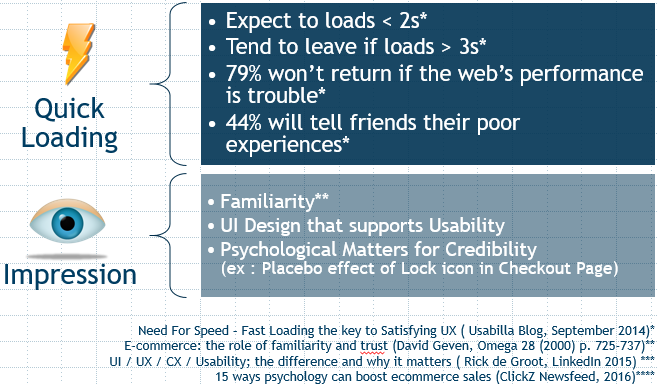
\includegraphics
	[width=.4\textwidth]
	{images/bab3/analisa/user-centered.png}
	\caption{Visualisasi aspek bisnis dalam \textit{software engineering}}
	\label{user-centered-analysis}
\end{figure}

Selain dari faktor \textit{user experience} dan \textit{performance}, beberapa hal yang menjadi poin penting dan menarik dalam beberapa studi yang terkait adalah sebagai berikut:
\begin{enumerate}[label=\alph*.]
	\item \textit{Familiarity} - yang dapat didefinisikan sebagai tingkat familier atau kesamaan dengan sistem sejenis ternyata dapat membangun \textit{trust} sehingga mensugesti pengguna untuk menyelesaikan transaksi yang dilakukan\cite{geven_e-commerce};
	\item \textit{Usability} yang memudahkan pengguna dalam menyelesaikan transaksi; dan
	\item Aspek-aspek psikologi seperti pemilihan warna, penggunaan \textit{icon} yang sesuai, seperti \textit{icon} gembok pada halaman pembayaran ternyata dapat mengesankan \textit{security} pada pengguna\cite{ewer_psychology_2014}\cite{coffin_color_2013}.
\end{enumerate}

\subsection{\textit{Technical Analysis}}
 Selain dari kualitas nilai jual aplikasi yang akan dibuat, ketahanan terhadap perubahan karena \textit{e-commerce} adalah sesuatu yang sangat cepat berubah karena kompetitor yang sangat kompetitif dan dorongan tehnologi yang membuat efektifitas dan efisiensi menjadi lebih baik.
Dari aspek \textit{software engineering} sendiri, \textit{software engineering} dimaksudkan untuk menunjang/\textit{support} pengembangan \textit{software} daripada \textit{individual programming}. Hal ini mencakup: \begin{inlinelist}
	\item \textit{evolution};
	\item \textit{design}; \textit{and}
	\item \textit{supporting program specification}
\end{inlinelist}\cite{software-engineering}.
Kebutuhan nonfungsional pada aplikasi ini didefinisikan pada Tabel 
%\captionsetup[table]{position=top,labelfont={sc},textfont={sl}}

\begin{table}[h!]
	\centering
	\caption{Kebutuhan Nonfungsional Aplikasi}
	\label{nonfung}
	\vfill
	\begin{tabular}{c|l|l}
		\hline
		\toprule
		No & Parameter & Keterangan\\ \hline
		\midrule
		1 & Ketersediaan & \textit{Available anytime via browser} \\ 
		2 & Bahasa & Menggunakan Bahasa Indonesia \\ 
		3 & Otorisasi & Otorisasi hak akses pengguna\\ 
		4 & Kecepatan & Waktu \textit{load} halaman kurang dari 3 detik \\ 
		5 & \textit{Positive User Experience} & Memberi kesan UX yang positif\\ 
		6 & \textit{Security} & Koneksi terlindung SSL/\textit{https}.\\ 
		7 & \textit{Maintainability} & Mudah di\textit{maintain}\\ 
		\bottomrule
	\end{tabular}
\end{table}

\subsection{Perancangan}	
	Sesuai definisi kebutuhan yang didefinisikan dalam \textit{paper}\cite{noauthor_application_2005}, kasus penggunaan aplikasi ini didefinisikan pada Gambar \ref{ucd.main}.
	\begin{figure}[h!]
		\centering
		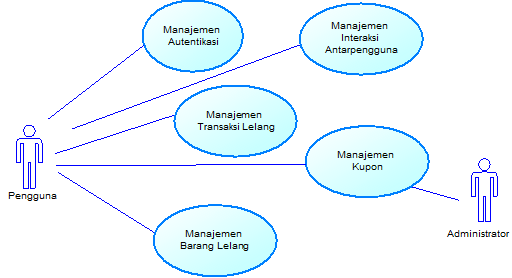
\includegraphics
		[width=.45\textwidth]
		{images/bab3/usecasediagram/ucd-main.png}
		\caption{Diagram Kasus Penggunaan Aplikasi}
		\label{ucd.main}
	\end{figure}
	Arsitektur fundamental diidentifikasi divisualisasikan pada Gambar \ref{fundamental-component} yaitu komponen-komponen penting dalam pembuatan aplikasi sebagai berikut.
	\begin{enumerate}
		\item Web Server 
		\item Mekanisme penyimpanan data (\textit{database} dan \textit{data storage})
		\item \textit{User Interface} sebagai media terhadap \textit{end-user}
		\item Mekanisme Asinkronus untuk mengakomodasi fitur \textit{realtime}
	\end{enumerate}
	
	\begin{figure}[h!]
		\centering
		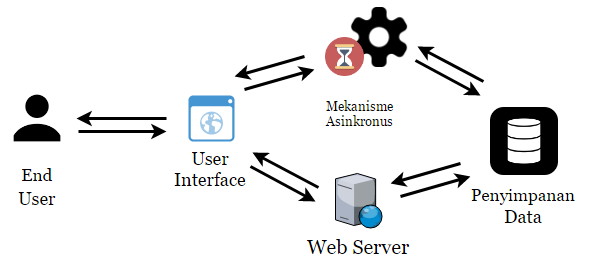
\includegraphics
		[width=.45\textwidth]
		{images/bab3/buku/basic_architecture.png}
		\caption{Arsitektur dasar yang dibutuhkan untuk membangun aplikasi}
		\label{fundamental-component}
	\end{figure}
	
	Digabungkan dengan kebutuhan fungsionalitas dan kelebihan kekurangan masing-masing teknologi pembangun yang ada, maka didefinisikan arsitektur lengkap dan pemilihan teknologi seperti pada gambar \ref{final-arch-tech-figure}.
	
	\begin{figure}[H]
		\centering
		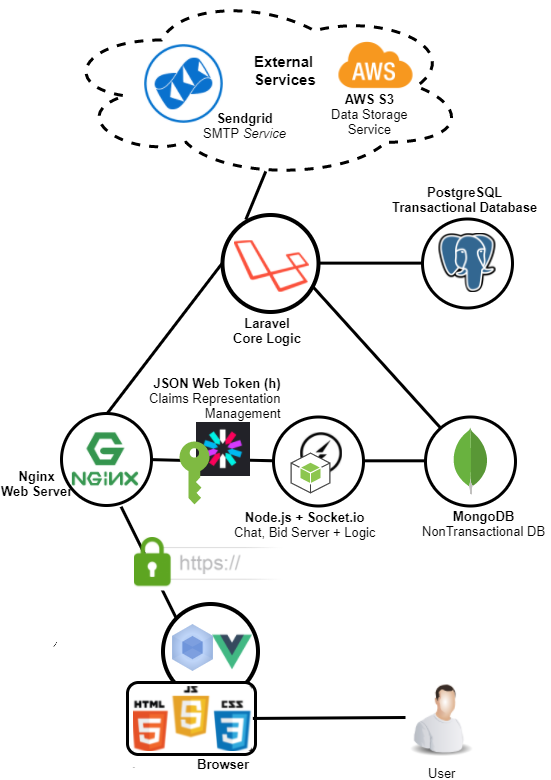
\includegraphics[width=.4\textwidth]{images/bab3/diagram-portrait.png}
		\caption{Visualisasi arsitektur dan teknologi Final yang diterapkan dalam rancang bangun aplikasi}
		\label{final-arch-tech-figure}
	\end{figure}
	
		
		Untuk mengakomodasi kebutuhan \textit{flexibility} dan \textit{maintainability}, maka penulis membangun aplikasi dengan menggunakan \textit{repository} pattern, dengan pembagian lingkup \textit{tiers} sebagai berikut:
		\begin{enumerate}
			\item \textit{Presentation tier}, bertanggungjawab terhadap tampilan dan \textit{view logic} di lingkup \textit{browser} pengguna;
			\item \textit{Bussiness tier}, merupakan \textit{logic} dari proses bisnis aplikasi;
			\item \textit{Integration tier}, merupakan integrasi manajemen pemrosesan data dan \textit{external services}; dan
			\item \textit{Resource tier}, bertanggung jawab terhadap \textit{data access layer}.
		\end{enumerate}
		\begin{figure}[]
			\centering
			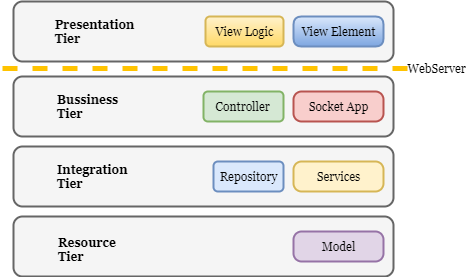
\includegraphics[width=.4\textwidth]{images/bab3/apl/main-apl.png}
			\caption{Visualisasi arsitektur dan teknologi Final yang diterapkan dalam rancang bangun aplikasi}
			\label{tiers}
		\end{figure}
\subsection{Deskripsi Sistem}
Aplikasi dapat diakses melalui \textit{browser} lewat URL {\url{https://lelangapa.com}}. Seperti \textit{e-commerce} pada umumnya, siapa saja dapat mendaftar ke dalam sistem sebagai dan memulai aktivitas lelang, baik sebagai pelelang maupun penjual barang.
\begin{figure}[h!]
	\centering
	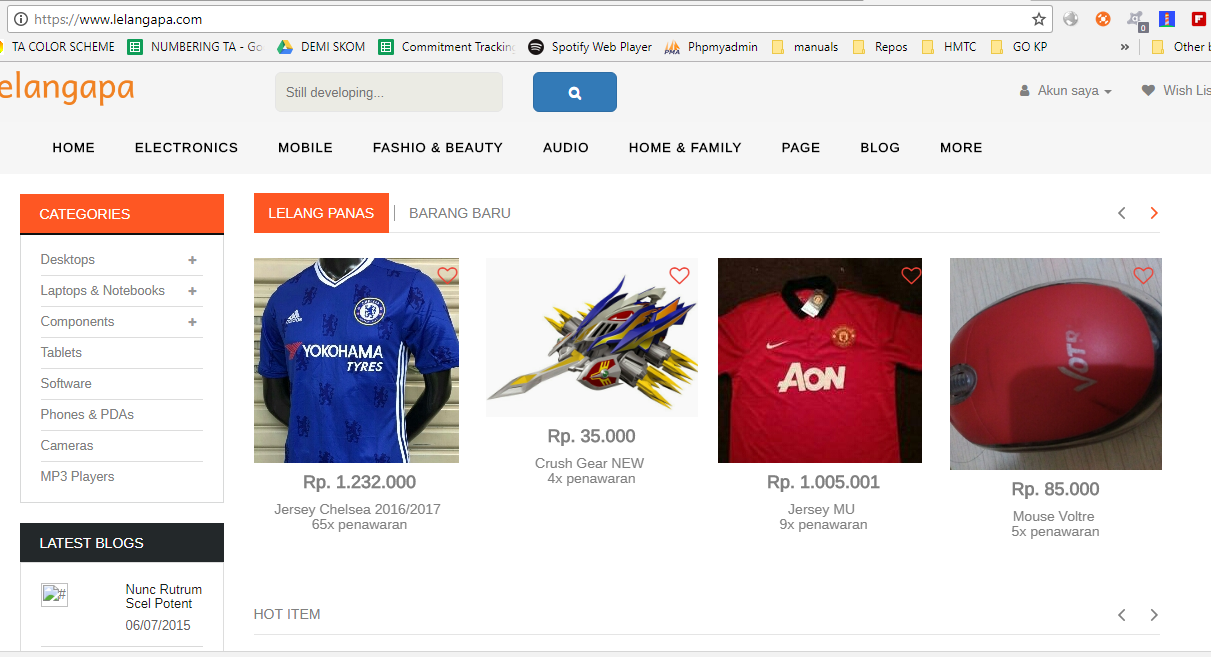
\includegraphics[width=.45\textwidth]{images/UI/landing.png}
	\caption{Tampilan \textit{landing page} aplikasi}
	\label{snap-landing}
\end{figure}
